% This file was created by tikzplotlib v0.9.8.
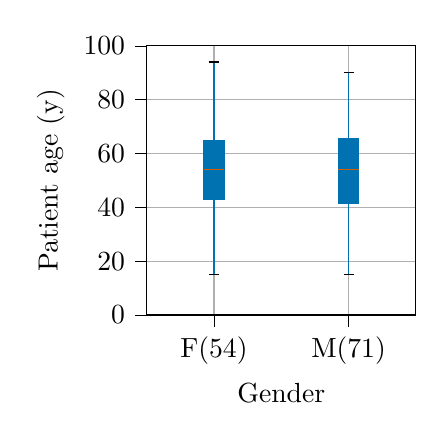
\begin{tikzpicture}

\definecolor{color0}{rgb}{0,0.447058823529412,0.698039215686274}
\definecolor{color1}{rgb}{0.835294117647059,0.368627450980392,0}

\begin{axis}[
height=5cm,
tick align=outside,
tick pos=left,
width=5cm,
x grid style={white!69.0196078431373!black},
xlabel={Gender},
xmajorgrids,
xmin=0.5, xmax=2.5,
xtick style={color=black},
xtick={1,2},
xticklabels={F(54),M(71)},
y grid style={white!69.0196078431373!black},
ylabel={Patient age (y)},
ymajorgrids,
ymin=0, ymax=100,
ytick style={color=black}
]
\addplot [color0, opacity=1]
table {%
1 42.75
1 15
};
\addplot [color0, opacity=1]
table {%
1 64.75
1 94
};
\addplot [black, opacity=1]
table {%
0.9625 15
1.0375 15
};
\addplot [black, opacity=1]
table {%
0.9625 94
1.0375 94
};
\addplot [color0, opacity=1]
table {%
2 41.5
2 15
};
\addplot [color0, opacity=1]
table {%
2 65.5
2 90
};
\addplot [black, opacity=1]
table {%
1.9625 15
2.0375 15
};
\addplot [black, opacity=1]
table {%
1.9625 90
2.0375 90
};
\path [draw=color0, fill=color0]
(axis cs:0.925,42.75)
--(axis cs:1.075,42.75)
--(axis cs:1.075,64.75)
--(axis cs:0.925,64.75)
--(axis cs:0.925,42.75)
--cycle;
\path [draw=color0, fill=color0]
(axis cs:1.925,41.5)
--(axis cs:2.075,41.5)
--(axis cs:2.075,65.5)
--(axis cs:1.925,65.5)
--(axis cs:1.925,41.5)
--cycle;
\addplot [color1, opacity=1]
table {%
0.925 54
1.075 54
};
\addplot [color1, opacity=1]
table {%
1.925 54
2.075 54
};
\end{axis}

\end{tikzpicture}
